\newpage
\section{Замена координат}\label{coords}

\subsection{Постановка задачи}\label{coords:task}

На плоскости или в пространстве заданы некоторые геометрические объекты в своем базисе. Необходимо найти координат этих объектов при замене базиса на новый.

\begin{figure}[h]
	{ \noindent \centering
	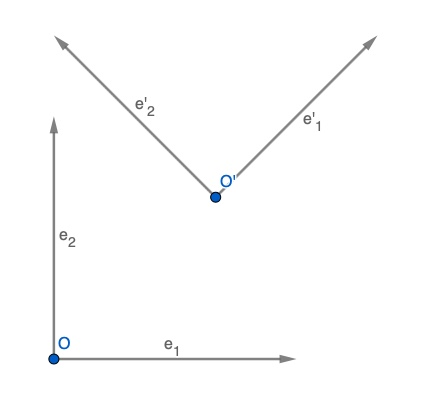
\includegraphics[scale=0.5]{cords2d}
	\caption{Два базиса на плоскости.}
	}
\end{figure}

\begin{figure}[h]
	{ \noindent \centering
	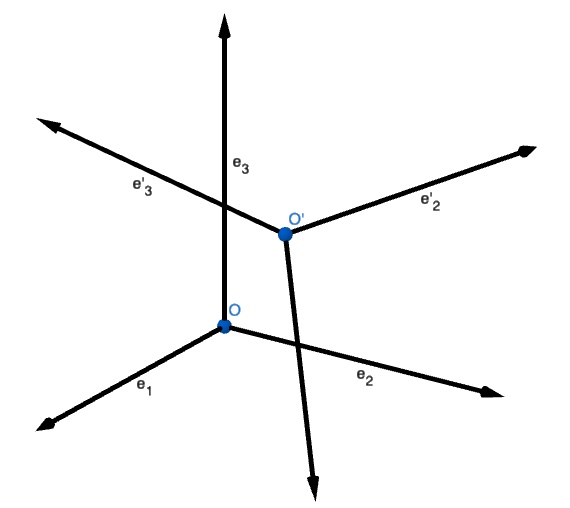
\includegraphics[scale=0.5]{cords3d}
	\caption{Два базиса в пространстве.}
	}
\end{figure}

\newpage
\subsection{Двумерный случай}\label{coords:alg:2dim}

Рассмотрим ортогональную матрицу как матрицу перехода от ортонормированного базиса $e_1, e_2$ к ортонормированному базису $e'_1, e'_2$. Тогда вектор $e'_1$ имеет координаты $(\cos \varphi, \sin \varphi)$ для некоторого $\varphi$. Перпендикулярные ему векторы единичной длины (таких два) равны $(\mp \sin \varphi, \pm \cos \varphi)$.\\

Таким образом, ортогональные матрицы 2x2 имеют один из следующих видов:
$$C = 
\begin{pmatrix}
	\cos \varphi & -\sin \varphi \\
	\sin \varphi & \cos \varphi
\end{pmatrix}, \; C = 
\begin{pmatrix}
	\cos \varphi & \sin \varphi \\
	\sin \varphi & -\cos \varphi
\end{pmatrix}$$

Угол $\varphi$ можно считать принадлежащим $[0, 2\pi)$.\\

Координаты точки в старой и новой с. к. связаны соотношениями:
$$\begin{pmatrix}
	x \\ y
\end{pmatrix} = C \begin{pmatrix}
	x' \\ y'
\end{pmatrix} + \begin{pmatrix}
	x_0 \\ y_0
\end{pmatrix}$$
где $C$ - матрица перехода от старого базиса к новому,

\hspace{0.4cm}$(x,y)$ и $(x', y')$ - координаты точки в старой и новой с.к.

\hspace{0.4cm}$(x_0, y_0)$ - координаты нового начала координат $O'$ в старой с.к.\\

Координаты векторов в старой и новой с. к. связаны соотношениями:
$$\begin{pmatrix}
	\alpha \\ \beta
\end{pmatrix} = C \begin{pmatrix}
	\alpha' \\ \beta'
\end{pmatrix}$$

Чтобы найти обратную замену, необходимо умножить на $C^{-1}$, а для ортогональных матриц $C^{-1} = C^T$. Таким образом:
$$\begin{pmatrix}
	x' \\ y'
\end{pmatrix} = C^T \begin{pmatrix}
	x \\ y
\end{pmatrix} - C^T \begin{pmatrix}
	x_0 \\ y_0
\end{pmatrix}$$

\newpage
\subsection{Трехмерный случай}\label{coords:alg:3dim}

Рассмотрим переход от прямоугольной системы координат $O e_1 e_2 e_3$ к другой прямоугольной системе координат $O e'_1 e'_2 e'_3$.

При коолинеарности одного из базисных векторов, например, $e_3$ первого репера и одного базисного вектора, например, $e'_3$ из второго репера замена сводится к замене координат на плоскости с определителем соответствующего знака в зависимости от направленности коллинерных векторов.

Теперь будем считать, что все векторы неколлинеарны, в частности, $e_3$ и $e'_3$ неколлинеарны:
$$\begin{gathered}
	e_3 \text{ - вектор нормали к плоскости } O e_1 e_2 \\
	e'_3 \text{ - вектор нормали к плоскости } O' e'_1 e'_2
\end{gathered}$$

Определим вектор $f := \frac{[e_3, e'_3]}{||[e_3, e'_3]||}$ - это направляющий вектор прямой пересечения плоскостей $O e_1 e_2$ и $O' e'_1 e'_2$.

Также определим \textit{углы Эйлера}:
\begin{itemize}
	\item[$\bullet$] угол $\varphi$ - это угол от $e_1$ к $f$, $\varphi \in [0, 2\pi)$
	\item[$\bullet$] угол $\theta$ - это угол от $e_3$ к $e'_3$, $\theta \in [0, \pi]$
	\item[$\bullet$] угол $\psi$ - это угол от $f$ к $e'_1$, $\psi \in [0, 2\pi)$
\end{itemize}

Будем последовательно производить замены координат: повороты в соответствующих плоскостях.

\begin{enumerate}
	\item Переход от $O e_1 e_2 e_3$ к $O f g e_3$ с сохранением ориентации - это вращение вокруг $e_3$ на угол $\phi$. Соответствующая матрица перехода имеет вид:
	$$C_1 = \begin{pmatrix}
		\cos \varphi & -\sin \varphi & 0 \\
		\sin \varphi & \cos \varphi & 0 \\
		0 & 0 & 1
	\end{pmatrix}$$
	\item Проведем вращение вокруг $f$ так, чтобы $e_3$ совместился с $e'_3$ - это вращение на угол $\theta$ (в силу определения $f$). Получаем переход к реперу $O f h e'_3$, причем плоскости $O f h$ и $O e'_1 e'_2$ совпадают. Соответствующая матрица перехода имеет вид:
	$$C_2 = \begin{pmatrix}
		1 & 0 & 0 \\
		0 &\cos \theta & -\sin \theta\\
		0 & \sin \theta & \cos \theta
	\end{pmatrix}$$
	\item Проведем вращение вокруг $e'_3$ в плоскости $O e'_1 e'_2$ для совмещения $f$ и $e'_1$. При этом в силу согласованности ориентаций образ $e_2$ перейдет в $e'_2$.
	Соответствующая матрица перехода имеет вид:
	$$C_3 = \begin{pmatrix}
		\cos \psi & -\sin \psi & 0 \\
		\sin \psi & \cos \psi & 0 \\
		0 & 0 & 1
	\end{pmatrix}$$
\end{enumerate}

Тогда результирущая матрица перехода от базиса $e_1 e_2 e_3$ к $e'_1 e'_2 e'_3$ равна:
$$\begin{gathered}
	C = C_1 C_2 C_3 = \begin{pmatrix}
		\cos \varphi & -\sin \varphi & 0 \\
		\sin \varphi & \cos \varphi & 0 \\
		0 & 0 & 1
	\end{pmatrix} 
	\begin{pmatrix}
		1 & 0 & 0 \\
		0 &\cos \theta & -\sin \theta\\
		0 & \sin \theta & \cos \theta
	\end{pmatrix}
	\begin{pmatrix}
		\cos \psi & -\sin \psi & 0 \\
		\sin \psi & \cos \psi & 0 \\
		0 & 0 & 1
	\end{pmatrix} = \\
	= \begin{pmatrix}
		\cos \varphi \cos \psi - \sin \varphi \cos \theta \sin \psi    &    - \cos \varphi \sin \psi - \sin \varphi \cos \theta \cos \psi    &     \sin \varphi \sin \theta \\
		\sin \varphi \cos \psi + \cos \varphi \cos \theta \sin \psi    &    - \sin \varphi \sin \psi + \cos \varphi \cos \theta \cos \psi    &     -\cos \varphi \sin \theta \\
		\sin \theta \sin \psi & \sin \theta \cos \psi & \cos \theta  
	\end{pmatrix}
\end{gathered}$$

Координаты точки в старой и новой с. к. связаны соотношениями:
$$\begin{pmatrix}
	x \\ y \\ z
\end{pmatrix} = C \begin{pmatrix}
	x' \\ y' \\ z'
\end{pmatrix} + \begin{pmatrix}
	x_0 \\ y_0 \\ z_0
\end{pmatrix}$$
где $C$ - матрица перехода от старого базиса к новому,

\hspace{0.4cm}$(x,y,z)$ и $(x', y', z')$ - координаты точки в старой и новой с.к.

\hspace{0.4cm}$(x_0, y_0, z_0)$ - координаты нового начала координат $O'$ в старой с.к.\\

Координаты векторов в старой и новой с. к. связаны соотношениями:
$$\begin{pmatrix}
	\alpha \\ \beta \\ \gamma
\end{pmatrix} = C \begin{pmatrix}
	\alpha' \\ \beta' \\ \gamma'
\end{pmatrix}$$

Чтобы найти обратную замену, необходимо умножить на $C^{-1}$, а для ортогональных матриц $C^{-1} = C^T$. Таким образом:
$$\begin{pmatrix}
	x' \\ y' \\ z'
\end{pmatrix} = C^T \begin{pmatrix}
	x \\ y \\ z
\end{pmatrix} - C^T \begin{pmatrix}
	x_0 \\ y_0 \\ z_0
\end{pmatrix}$$

